
\lecture{8}{The Second Law and Entropy}{Qiang Zhu}{scribe-name1,2,3}


\section{Entropy}
\begin{equation} \label{entropy} 
S = k \text{ln}\Omega 
\end{equation}

\section{Entropy of Einstein Solid}
\begin{equation} \label{entropy} 
S = k\text{ln}(eq/N)^N = Nk[\text{ln}(q/N)+1]
\end{equation}
if $N$=\textrm{$10^{22}$}, $q$=\textrm{$10^{24}$}
\begin{equation} \label{entropy} 
S = Nk(~~~~~~~~~~~~~~~~~)= ~~~~~~~~~~~~~\text{J/K} 
\end{equation}

\begin{enumerate}
\item Discuss the relation between $S$ and $q$, $N$?
\item Mixing A and B?
\item Entropy tends to increase?
\end{enumerate}

{\bf Exercise} \\
Based on Figure 2.5, compute the entropy of the total, most likely, least likely macrostate. Compare them with the number of typical values (0.77J/K).

\section{Entropy of an Ideal Gas}
\begin{equation} \label{entropy} 
S = Nk[\text{ln}(\frac{V}{N} (\frac{4\pi m U}{3Nh^2})^{3/2}) + \frac{5}{2}]
\end{equation}

This is called the \textbf{Sackur-Tetrode equation}.

\begin{enumerate}
\item Discuss the relation between $S$ and $V$, $N$, $m$, $U$, compare it with Einestein solid?
\item Compute $S$ for He/Ar? (Same $N$, $V$, $U$, with a radius of the hypersurface of $P$ is $\sqrt{2mU}$ ) 
\item Free expansion? How to calculate $\Delta{S}$, with an alternative way?
\end{enumerate}

\begin{figure}[h]
\centering
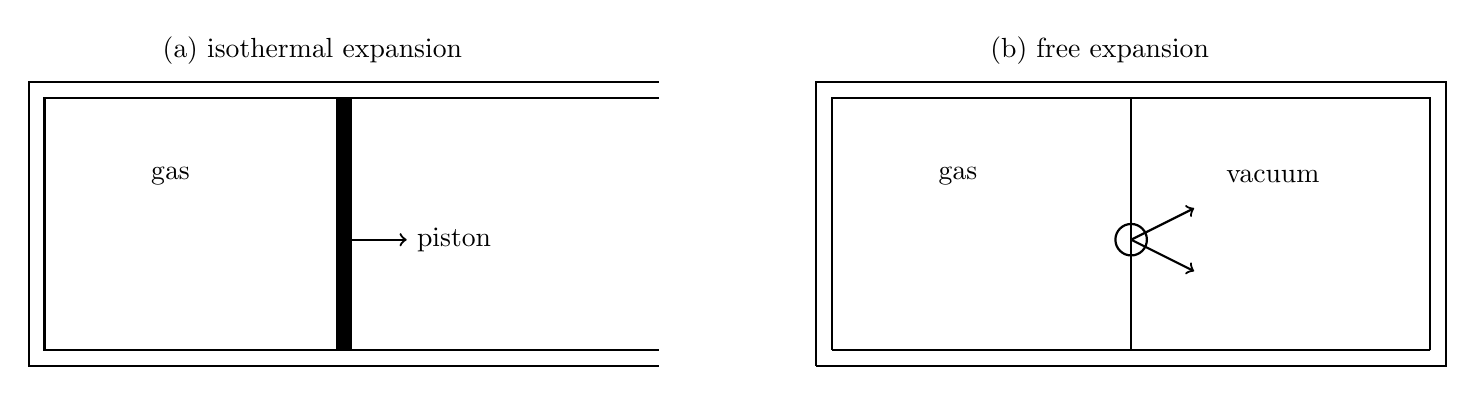
\begin{tikzpicture}[thick]
\draw (8,4) -- (0,4) -- (0,0.4) -- (8,0.4);
\draw (8,3.8) -- (0.2,3.8) -- (0.2,0.6) -- (8,0.6);
\draw [line width=0.2cm](4,3.8) -- (4,0.6); 
\draw [->](4,2) -- (4.8,2) node[right]{piston}; 
\node at (1.8,2.8) {gas};
\node at (3.6,4.4) {(a) isothermal expansion};

\draw (10,0.4) -- (18,0.4) -- (18,4) -- (10,4) -- (10,0.4);
\draw (10.2,0.6) -- (14.0,0.6) -- (14.0,3.8) -- (10.2,3.8) -- (10.2,0.6);
\node at (11.8,2.8) {gas};
\draw (17.8,0.6) -- (14.0,0.6) -- (14.0,3.8) -- (17.8,3.8) -- (17.8,0.6);
\node at (15.8,2.8) {vacuum};
\node at (13.6,4.4) {(b) free expansion};
\draw [->] (14,2) -- (14.8,2.4);
\draw [->] (14,2) -- (14.8,1.6);
\draw (14,2) circle (0.2cm);
\end{tikzpicture}
\end{figure}


\section{Mixing Entropy of an Ideal Gas}
If we mix two different gases, A and B, each with the same $U$, $V$ and $N$, they occupy two halves of a divided chamber.
\begin{equation}\Delta S_A = Nk\text{ln} V_f/V_i = Nkln2 \end{equation}
\begin{equation}\Delta S_B = Nk\text{ln} V_f/V_i = Nkln2 \end{equation}
\begin{equation}\Delta S_\text{total} = 2Nkln2 \end{equation}

What if $A$ and $B$ are indistinguishable? (double counting?)
Mixing only applies when $A$ and $B$ are different?
\begin{figure}[h]
\centering
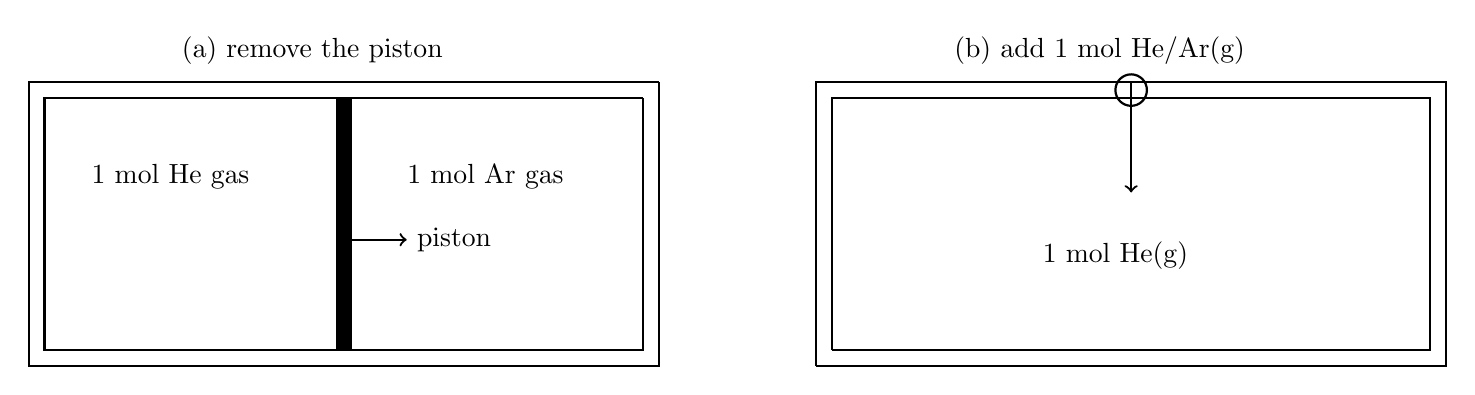
\begin{tikzpicture}[thick]
\draw (8,4) -- (0,4) -- (0,0.4) -- (8,0.4) -- (8,4);
\draw (7.8,3.8) -- (0.2,3.8) -- (0.2,0.6) -- (7.8,0.6) -- (7.8,3.8);
\draw [line width=0.2cm](4,3.8) -- (4,0.6); 
\draw [->](4,2) -- (4.8,2) node[right]{piston}; 
\node at (1.8,2.8) {1 mol He gas};
\node at (5.8,2.8) {1 mol Ar gas};
\node at (3.6,4.4) {(a) remove the piston};


\draw (10,0.4) -- (18,0.4) -- (18,4) -- (10,4) -- (10,0.4);
\draw (10.2,0.6) -- (17.8,0.6) -- (17.8,3.8) -- (10.2,3.8) -- (10.2,0.6);
\node at (13.8,1.8) {1 mol He(g)};
\draw [-> ](14,4.0) -- (14,2.6);
\node at (13.6,4.4) {(b) add 1 mol He/Ar(g)};
\draw (14,3.9) circle (0.2cm);
\end{tikzpicture}
\end{figure}


\section{Irreversible process}
\begin{enumerate}
\item Entropy increase $\rightarrow$ irreversible
\item Entropy unchanged $\rightarrow$ reversible
\item Slow compression, quasi static, reversible
\item Heat flow is always irreversible
\item Mixing (+$V$), stir salt in to soup, scrambling egg
\item +$N$, Burning gasoline, large molecule to small molecules, Cut down a tree
\end{enumerate}

\ce{CH4(gas) + 2O2(gas) -> CO2(gas) + 2H2O(gas)} ~~~~~~~S\\
\ce{2H2(gas) + O2(gas) -> 2H2O(gas)}~~~~~~~~~~~ S\\
If you consider it is not a isolated system. It also produces heat, so the total entropy is increasing due to heat.

\section{Homework}
Prove that 1 mol Ar gas has larger entropy than 1 mol He.\\
Problems 2.17, 2.18, 2.22, 2.29, 2.30, 2.31, 2.32, 2.34, 2.37


